%\documentclass[journal]{vgtc}                % final (journal style)
\documentclass[review,journal]{vgtc}         % review (journal style)
%\documentclass[widereview]{vgtc}             % wide-spaced review
%\documentclass[preprint,journal]{vgtc}       % preprint (journal style)
%\documentclass[electronic,journal]{vgtc}     % electronic version, journal

%% Uncomment one of the lines above depending on where your paper is
%% in the conference process. ``review'' and ``widereview'' are for review
%% submission, ``preprint'' is for pre-publication, and the final version
%% doesn't use a specific qualifier. Further, ``electronic'' includes
%% hyperreferences for more convenient online viewing.

%% Please use one of the ``review'' options in combination with the
%% assigned online id (see below) ONLY if your paper uses a double blind
%% review process. Some conferences, like IEEE Vis and InfoVis, have NOT
%% in the past.

%% Please note that the use of figures other than the optional teaser is not permitted on the first page
%% of the journal version.  Figures should begin on the second page and be
%% in CMYK or Grey scale format, otherwise, colour shifting may occur
%% during the printing process.  Papers submitted with figures other than the optional teaser on the
%% first page will be refused.

%% These three lines bring in essential packages: ``mathptmx'' for Type 1
%% typefaces, ``graphicx'' for inclusion of EPS figures. and ``times''
%% for proper handling of the times font family.

\usepackage{mathptmx}
\usepackage{graphicx}
\usepackage{times}
\usepackage{epstopdf}

%% We encourage the use of mathptmx for consistent usage of times font
%% throughout the proceedings. However, if you encounter conflicts
%% with other math-related packages, you may want to disable it.

%% This turns references into clickable hyperlinks.
\usepackage[bookmarks,backref=true,linkcolor=black]{hyperref} %,colorlinks
\hypersetup{
  pdfauthor = {},
  pdftitle = {},
  pdfsubject = {},
  pdfkeywords = {},
  colorlinks=true,
  linkcolor= black,
  citecolor= black,
  pageanchor=true,
  urlcolor = black,
  plainpages = false,
  linktocpage
}

%% If you are submitting a paper to a conference for review with a double
%% blind reviewing process, please replace the value ``0'' below with your
%% OnlineID. Otherwise, you may safely leave it at ``0''.
\onlineid{153}

%% declare the category of your paper, only shown in review mode
\vgtccategory{Research}

%% allow for this line if you want the electronic option to work properly
\vgtcinsertpkg

%% In preprint mode you may define your own headline.
%\preprinttext{To appear in an IEEE VGTC sponsored conference.}

%% Paper title.

\title{Chameleon: Dynamic Color Mapping	for Multi-Scale Structural Biology Models}

%% This is how authors are specified in the journal style

%%% indicate IEEE Member or Student Member in form indicated below
\author{Nicholas Waldin}
%\author{Roy G. Biv, Ed Grimley, \textit{Member, IEEE}, and Martha Stewart}
%\authorfooter{
%%% insert punctuation at end of each item
%\item
% Roy G. Biv is with Starbucks Research. E-mail: roy.g.biv@aol.com.
%\item
% Ed Grimley is with Grimley Widgets, Inc.. E-mail: ed.grimley@aol.com.
%\item
% Martha Stewart is with Martha Stewart Enterprises at Microsoft
% Research. E-mail: martha.stewart@marthastewart.com.
%}

%other entries to be set up for journal
%\shortauthortitle{Biv \MakeLowercase{\textit{et al.}}: Global Illumination for Fun and Profit}
%\shortauthortitle{Firstauthor \MakeLowercase{\textit{et al.}}: Paper Title}

%% Abstract section.
\abstract{
%	Visualizations of biological structures across multiple scales are becoming popular as more and more detailed data from the atomic level up to the cellular level are becoming available. To support seamless interactive exploration of such models, visual representations of elements on different levels of detail are necessary. While multi-scale structural representations have been extensively explored in the past (?), we address a new challenge introduced in multi-scale visualizations covering several orders of magnitude, namely multi-scale color coding. Categorical color coding is essential for identification of structures, but their usage varies with the level of detail from the visualization, from encoding atom types to compartments of a cell. 

Visualization of structural biology data uses color to categorize or separate dense structures into particular semantic units. In multiscale models of viruses or bacteria, there are atoms on the finest detail, aminoacids, secondary structures, macromolecules, up to the compartment level and all these levels can be visually distinguished by color. However, currently only a single scale coloring schemes are utilized that show information for that particular scale only. We present a novel technology which adaptively, based on a current scale level, adjusts the color scheme to depict or distinguish the currently best visible structural information. We treat the color as a visual resource that is distributed given a particular demand. The changes of the color scheme are seamlessly interpolated between the color scheme from the previous views into a given new one. With such dynamic multi-scale color mapping we ensure that the viewer is able to distinguish structural detail that is shown to her on a given scale. This technique has been tested on subjects with an expertise in structural biology and has been overall well received.

} % end of abstract

%% Keywords that describe your work. Will show as 'Index Terms' in journal
%% please capitalize first letter and insert punctuation after last keyword
\keywords{Bla, Bla, Bla}

%% ACM Computing Classification System (CCS). 
%% See <http://www.acm.org/class/1998/> for details.
%% The ``\CCScat'' command takes four arguments.

\CCScatlist{ % not used in journal version
 \CCScat{K.6.1}{Management of Computing and Information Systems}%
{Project and People Management}{Life Cycle};
 \CCScat{K.7.m}{The Computing Profession}{Miscellaneous}{Ethics}
}

%% Uncomment below to include a teaser figure.
  \teaser{
 \centering
 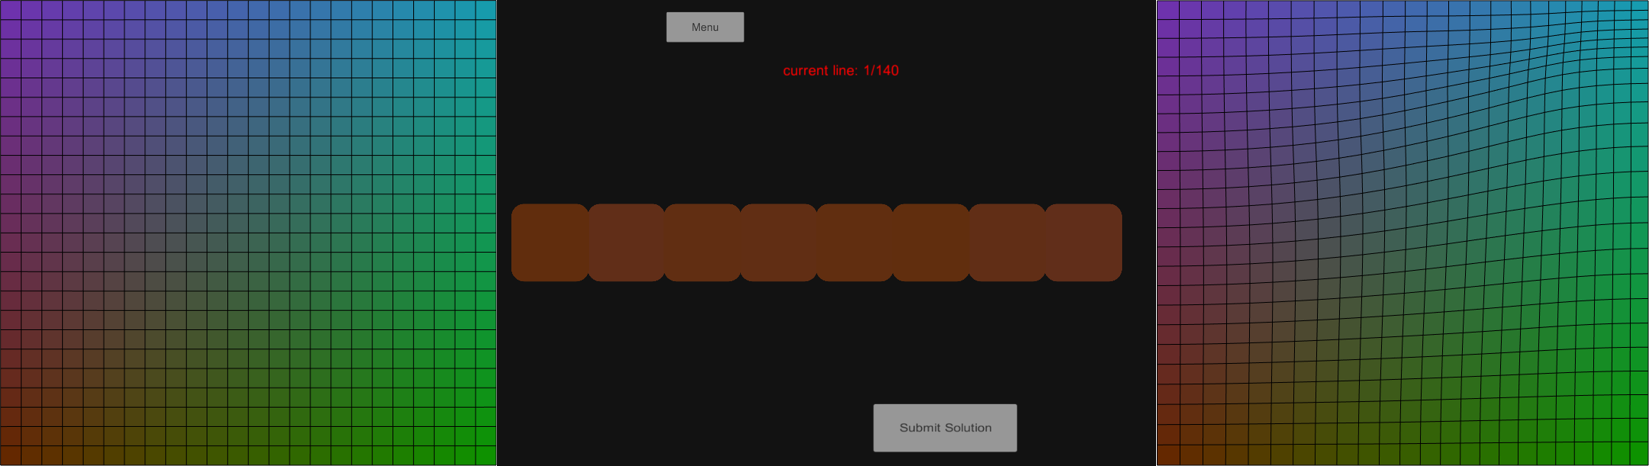
\includegraphics[width=16cm]{Figures/Picture1.png}
  \caption{In the Clouds: Vancouver from Cypress Mountain.}
  }

%% Uncomment below to disable the manuscript note
\renewcommand{\manuscriptnotetxt}{}

%% Copyright space is enabled by default as required by guidelines.
%% It is disabled by the 'review' option or via the following command:
% \nocopyrightspace

%%%%%%%%%%%%%%%%%%%%%%%%%%%%%%%%%%%%%%%%%%%%%%%%%%%%%%%%%%%%%%%%
%%%%%%%%%%%%%%%%%%%%%% START OF THE PAPER %%%%%%%%%%%%%%%%%%%%%%
%%%%%%%%%%%%%%%%%%%%%%%%%%%%%%%%%%%%%%%%%%%%%%%%%%%%%%%%%%%%%%%%%

\begin{document}

%% The ``\maketitle'' command must be the first command after the
%% ``\begin{document}'' command. It prepares and prints the title block.

%% the only exception to this rule is the \firstsection command
\firstsection{Introduction}

\maketitle

%% \section{Introduction} %for journal use above \firstsection{..} instead

Biological organisms can be viewed on different scales. For example, the human body consists of organs, cells, proteins and molecules. As more detailed data is becoming available across all levels, it is possible to combine visualizations of multiple scale levels into a single integrated visual environment. This poses new challenges for visualization experts, including seamlessly adapting the levels of detail of structural representations for real-time rendering, .... (experts, please address the challenges). \newline
A challenge which has not been addressed so far is color-coding. Consider, for instance, the human immunodeficiency virus (HIV). To understand its viral lifecycle, researchers are investigating the shape of its compartments, the role of the individual proteins in viral replication, the secondary structures, as well as structural properties of binding sites on the atomic level. Traditionally, researchers use dedicated visual representations for each level of scale, and illustrators provide hand-crafted visualizations to communicate new findings to the general public. Each of these scale levels uses a distinct color coding so that observers are able to distinguish and identify the structures. Can we show existing examples here? \newline
When integrating multiple scales into a single zoomable visualization, it is therefore necessary to not only provide a seamless structural zooming, but also a color-coding mechanism that takes the current level of detail into account. While successively providing more levels of detail of the structures when zooming in, we are severely limited in the number of available colors due to perceptual constraints and limitations of the monitor hardware. \newline

We propose a semantic zooming method for visualizing color-coded a virusmulti-scale visualization based on a view- dependent hierarchical color-scheme. Starting from the lowest zoom-level, we iteratively split up the available color space to the number of necessary colors defined by the current zoom level and item visibility. Our method thereby trades discriminability of individual elements against temporal coherence. In the HIV example (refer to teaser image), the user initially sees the different compartments. As the user zooms in, the proteins receive more distinct colors based on which compartment they are in. As compartments and proteins disappear, the colors of the visible proteins are adjusted to enhance discernibility.  As the viewer zooms further in, the domains of the proteins will become distinct, and eventually even the atoms, whose colors are predefined by convention. 

\section{Related Work}

Color maps are used often in visualization. Their structure depends heavily on the application, as has been shown in [Colour for Presentation Graphics], [Color Design for Illustrative Visualization], A Rule-based Tool for Assisting Colormap Selection, http://ultra.sdk.free.fr/docs/Image/Colors/ARule-basedToolfo0AssistingColormapSelection.htm], [Choosing Effective Colours for Data Visualization], [a survey and task-based quality assessment of static 2d colormaps], [explorative analysis of 2d color maps]. Several tools have been developed to assist users select appropriate color maps, such as colorbrewer, or iwanthue, [http://tools.medialab.sciences-po.fr/iwanthue/] and XCluSim, which are aimed at generating colors for clusters of data. Such clustering can, however, cause perceptual issues, either due to the large number of clusters or their layout. Particular care needs to be taken when dealing with higher dimensional data [revisiting perceptually optimized color mapping for high dimensional data analysis], so the distances between the clusters do not become distorted. Furthermore, in cases such as coloring maps, visually dominant structures may visually suppress small groups or areas [Perceptually Driven Visibility Optimization for Categorical Data Visualization]. Recognition may also be affected by contrast effects which may need to be dealt with [Methods for Compensating Contrast Effects in Information Visualization].
XCluSim’s uses a tree based method [tree based method] that attempts to overcome these issues in the case of hierarchical structures. The tree method uses HCL space – a cylindrical coordinate version of CIELab with Hue , Chroma (Saturation), and Luminance – and gives each cluster a different hue. The root of the tree has no chroma, i.e. grey, and the hue is divided up into different sections, one for each branch, with some space cut out between branches, in order for there to be a jump in color from one section to another. As the tree spreads out, the chroma of the nodes increases, and each level gets its own smaller subsection. 
Sometimes hierarchical data can also be viewed on multiple levels at once, for example a protein can be viewed on the overall structure as well as on the atomic structure [Rendering Molecular Surfaces using Order-Independent Transparency]. Alternatively, distortions of the object or different rendering levels in different areas of the camera may be used. For example, in [A Rendering Framework for Multiscale Views of 3D Models] the area in the center of the camera is rendered as closer in. This is achieved through…. . Parts of the object can also be distorted, by example through widgets such as in [Non-linear perspective widgets for creating multiple-view images] or [Vessel visualization using curvicircular feature aggregation]. In the first case X, in the second case Y.

Level of detail and abstraction may also depend on the distance from the object.[ View-dependent level-of-detail abstraction for interactive atomistic visualization of biological struct] [Illustrative Molecular Visualization with Continuous Abstraction] [Illustrating the Machinery of Life: Viruses Continuous Levels-of-Detail and Visual Abstraction for Seamless Molecular Visualization]. 
These kinds of visualizations have to deal with two major problems. First is when to show which level and how many levels to show at once. An example of this is [A Rendering Framework for Multiscale Views of 3D Models] by x, where they show a method of showing different levels of detail of a human body. In our case, we don’t want to allow for distortion, as most of the items are a) fairly small, b) should be comparable to other elements nearby without distortion, and c) the user does not want to see all layers at once, as the structure of a protein holds little information about the structure of a cell.

\subsection{Molecular Visualization}

\section{Technique}

When applying a coloring scheme to data of this type, several things need to be taken into account. First, the representation should support the level the user is looking at, e.g. not show the protein domains when the user is looking at the compartment level. Second, switching from one level to another should not be confusing. Third, the user should be able to easily identify useful information at the level he is looking at. Because predetermining all the colors for each item in the scene and not allowing for view dependency will, with enough data, guarantee that data points will become indistinguishable. Fourth, the coloring must allow the user remain orientated and determine what belongs to the stuff he is interested in. For example, he needs to know where a compartment ends and the next one begins.
Stress the fact that temporal coherence and discriminability by color are contradicting each other if we need a lot of colors (give numbers for HIV!). 
Ware (?) points out that luminance is more useful for encoding high-frequency information, while hue is easier to interpret for encoding low-frequency information. This is also reflected in the well-known ColorBrewer color schemes, where colors of categorical palettes differ primarily by hue, while quantitative color schemes operate mostly on luminance level.  We therefore use utilize the HCL color space that separates these two properties into different dimensions (luminance is the vertical axis, while hue and chroma are represented on the perpendicular planes as polar coordinates). Another useful aspect of the HCL color space is that it is simply an alternative representation of the CIEL*a*b* color space and therefore perceptually linear. This means that we can linearly link changes in the color space to perceptual responses. 
We start by assigning each item on the lowest LOD a distinct hue. Since the lowest hierarchy level comprises the entire model, this assignment is static and does not change with the viewing angle. Given the number of elements $n$ on the lowest LOD, the desired luminance and chroma, the hue of the i’th element is simply defined by $h_i=i*360/n$. This results in $n$ isoluminant colors with equidistant hues. 
(Chroma is luminance-depending if we consider the sRGB boundaries, but we don’t do this now!)
We use a hue circle here, but any parametric curve within the HCL space could be used. In this case, the colors would not be isoluminant, but still equidistant in the perceptually linear color space. 
Each section applies force on its neighbouring section, proportional to the number of different kinds of proteins that are visible. This means that the section can grow and shrink, depending on visibility. If a compartment is not visible, then the section shrinks to a size zero. 

However, a degree of consistency is still desired. It would be unwanted for a compartment to switch over to the opposite color, such as blue to yellow.  As such something needs to be in place to keep compartments from moving too far.
The switch to the proteins color occurs when the distance is greater than 5*2.3 =5*jnd in cielab space [Mahy 94 evaluation after adoption]. This is equal to an angle of X on the hue circle.

Another problem is how do we choose the colors for the domains? Their color needs to be view dependent as well as near to the color of the protein they belong to. The color of the chains does not  
Interact with the color of the other proteins, but does if they are showing their chains. 
Whether or not the chains are shown depends on the how close the camera is to the protein, unless the color distance would be below a certain amount (5*2.3) (8.8 degrees). The hue circle is reused to show the colors of the chains. See fig[]. The chains don’t cause any force on the proteins, and the proteins cause no force on the chains. The chains of two different proteins can cause force on one another if they are being shown. Because the chains would normally surround the entire circle, they only push each other away to a maximum distance of X. This allows for the chains to have similar colors to the proteins.


\section{User study}
We opted to perform a qualitative evaluation with XX biologists consisting of two blocks. In the first block, users had to identify a set of pre-defined structures across multiple levels of scale in the HIV model. In the second block, users could freely explore the scene. In both blocks, users were encouraged to “think aloud”. Sessions were observed by one to two study administrators, the screen was captured, and audio was recorded. The session was concluded by a questionnaire and an audio-recorded semi-structured interview. 
The task was provided by a professor of molecular biology and well-known illustrator of biological models. Users were first provided by a description of the HIV capsid protein, which is the single protein building up the HIV capsid. Then they were asked to identify structures from this description in the HIV visualization, namely the capsid compartment itself, a special protein compound of the capsid, the two protein domains, secondary structures acting as binding sites, and a dedicated amino acid. 
The study was conducted on a (laptop specification, screen, color calibration). Users were sitting approximately ... cm from the screen, but were free to move. 
Before performing the actual study task, users were demonstrated how to navigate in the scene, and how to switch on and off certain sub-compartments. This was necessary so that all items were accessible without occlusions. 
We decided to perform a qualitative evaluation as our visualization is new, and there is currently no visualization that allows the user to look at all levels in a similar manner, so we do not have a method of comparison. Our goal primarily was to see whether domain experts can identify the individual structures, whether this would be possible without color coding at all, and whether the view-dependent color assignment was irritating for them. 

Users
The users were molecular biology students. As such, they had some but limited knowledge of the field [tbd may be variation]. As such, there needed to be an explanation of what they were looking for. The students ranged from x to y years studying.

Results
-	How many students found the different targets
-	Insights
-	Probably need table of different types of insights.
-	Insights per minute  (ipm)
-	Answer to the questions we pose (table?)
-	People used
-	Number of people used
-	Describe type of study
-	Describe what this kind of study is.
-	Reference other (similar) studies
-	Argue why 
o	No baseline
o	No quantifiability (x in y seconds)
o	Want to measure usability


\section{Conclusion}

Conclusion goes here.

%% if specified like this the section will be committed in review mode
\acknowledgments{
The authors wish to thank A, B, C. This work was supported in part by
a grant from XYZ.}

\bibliographystyle{abbrv}
%%use following if all content of bibtex file should be shown
%\nocite{*}
\bibliography{Chameleon}
\end{document}
